\section{States, parameters and dimensions}
States are denoted by $\mathbf{x}$ and stand for the unknowns of the power flow, such as the voltage magnitude. The traditional power flow looks to obtain a solution for all states; in the parametric power flow, this is not necessarily the case, as there might be only one bus under study. 

Parameters are defined as the input data which are meant to vary. Powers are part of this category, since loads change over time and most generation sources also experience variations. Considering a total of $m$ parameters, grouped under $\mathbf{p} = [p_1, p_2, ..., p_m]$, each parameter $p_k \ \forall k \in \{1, ..., m\}$ takes values inside the $[a_k, b_k]$ range. 

This way, the power flow problem can be written as:
\begin{equation}
  \mathbf{f}(\mathbf{x}, \mathbf{p}) = 0,
  \label{eq:power1}
\end{equation}
where $\mathbf{f}$ symbolizes all implicit functions involved in the solution of the problem. The formulation that follows is generic, in the sense that the methodology would be equally valid for other problems. Hence, this technique is not limited to the traditional power flow. 

The parametric approach looks to express a certain state as a function of the parameters:
\begin{equation}
  x = g(\mathbf{p}), 
  \label{eq:param1}
\end{equation}
where $g$ is a function pending to be found. 

From \eqref{eq:param1} it becomes clear that all parameters will potentially affect a given state. Visually speaking, Fig. \ref{fig:1ax}.a shows a representation of a state as a function of a single parameter, that is, assuming that only one input changes. Fig. \ref{fig:1ax}.b presents a similar visualization with two parameters involved. This justifies why, when viewed as a spatial representation, parameters are also denoted as dimensions. Each one of them stands for a new axis independent axis, and thus, orthogonal to the rest. 

% \begin{figure}[!htb]

%   \begin{subfigure}{0.49\textwidth}
%     \incfig{p1_1}
%     \caption{one-axis representation}
%   \end{subfigure}
%   \hspace*{\fill}
%   \begin{subfigure}{0.49\textwidth}
%     \incfig{p2_1}
%     \caption{two-axis representation}
%   \end{subfigure}

%   \caption{Representation of a state with one or two parameters}
%   \label{fig:1ax}
% \end{figure}

\begin{figure}[!htb]
\begin{subfigure}{0.4\textwidth}
  \vspace{1.13cm}
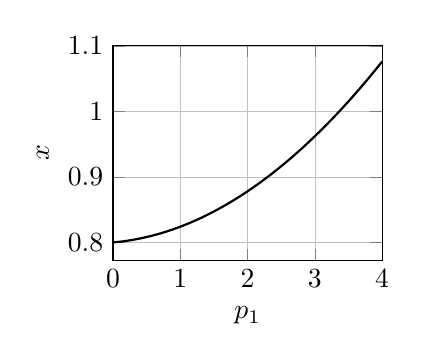
\begin{tikzpicture}
  \begin{axis}[xlabel={$p_1$}, ylabel={$x$}, grid=both, grid style={line width=.1pt, draw=gray!10}, major grid style={line width=.2pt,draw=gray!50}, xtick distance = 1, ytick distance = 0.1, width=5cm, every plot/.append style={very thick}, xmin = 0, xmax = 4]
\addplot [
    style=thick,
    domain=0:4,
    samples = 200] 
    {0.03 * (0.5 * x^2 + 0.3 * x) + 0.8};
\end{axis}
\end{tikzpicture}
\caption{one-axis representation}
\end{subfigure}
  \hspace{0.2cm}
\begin{subfigure}{0.6\textwidth}
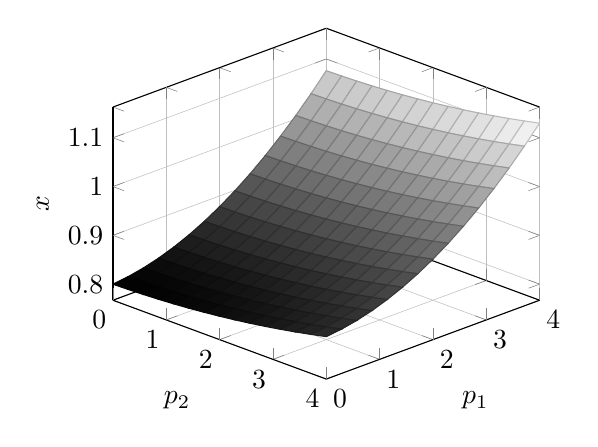
\begin{tikzpicture}
  \begin{axis}[colormap/blackwhite, xlabel={$p_2$}, ylabel={$p_1$}, zlabel={$x$}, grid=both, grid style={line width=.1pt, draw=gray!10}, major grid style={line width=.2pt,draw=gray!50}, xtick distance = 1, ytick distance = 1, ztick distance = 0.1, view={45}{30}, width=7cm]
\addplot3 [
    domain=0:4,
    domain y = 0:4,
    samples = 15,
    samples y = 15,
    surf] {0.03 * (0.5 * y^2 + 0.3 * y + 0.1 * x^2 + 0.05 * x) + 0.8};
\end{axis}
\end{tikzpicture}
\caption{two-axis representation}
\end{subfigure}
\caption{Representation of a state with one or two parameters}
\label{fig:1ax}
\end{figure}

More than two dimensions are expected to be present in a typical analysis of the parametric power flow. In a mid-size system, assuming all powers are treated as parameters, there could be hundreds of dimensions. If $m \approx 100$, opting for the naive approach with $n^m$ cases would be painful to compute. This is often called the curse of dimensionality. 

One fundamental step to circumvent this challenge is to reduce the dimensions. Note that in Fig. \ref{fig:1ax} the value of $x$ is more or less the same in both Fig. \ref{fig:1ax}.a and Fig. \ref{fig:1ax}.b. That is, $p_1$ has a larger influence than $p_2$. The essence of dimensionality reduction lies in compacting all dimensions into a few. A prerequisite is to determine the impact all parameters have on the state.  

\section{Principal Component Analysis}
The Principal Component Analysis (PCA) weights the parameters according to their influence. To do so, the first step is concerned with computing the gradient:
\begin{equation}
  \nabla_{\mathbf{p}}g = \left[\frac{\partial x}{\partial p_1}, ..., \frac{\partial x}{\partial p_k}, ..., \frac{\partial x}{\partial p_m} \right]^T.
  \label{eq:grad1}
\end{equation}
Calculating the gradient numerically is probably the most benefitial option because it allows to operate with implicit functions, just like the power flow is commonly presented. Hence, for all $k$ in $[1,...,m]$:
\begin{equation}
  \frac{\partial x}{\partial p_k} = \frac{g(p_1,...,p_k + \delta,...,p_m) - g(p_1,...,p_k,...,p_m)}{\delta},
  \label{eq:grad2}
\end{equation}
where $\delta$ is an arbitrary small number, such as $\delta=1\cdot 10^{-10}$ for instance. Computing the gradient with this approach means that the power flow solver has to be called $m+1$~times. 

Let $\mathbf{C}\in \mathbb{R}^{m \times m}$ be the covariance matrix. Its elements identify the influence of the parameters on the states. Large elements represent that the two involved parameters have a significant impact on the state, whereas small elements that these two parameters are potentially irrelevant. Since a parameter $k$ can take any value inside its corresponding range $[a_k,b_k]$, several samples have to be extracted to have a representative $\mathbf{C}$ matrix:
\begin{equation}
  \mathbf{C} \approx \frac{1}{M} \sum_{i=1}^M \nabla_{\mathbf{p}}g (\nabla_{\mathbf{p}}g)^T,
  \label{eq:C1}
\end{equation}
where $M$ is the total number of samples and takes a relatively arbitrary value. 

The parameters take random values in each sample. The power flow solver would have to be called $M(m+1)$ times in total. Although it largerly depends on the number of initial dimensions, $M$ can take values in the order of a hundred. As a consequence, it can be foreseen that calculating $M(m+1)$ power flows is generally way faster than computing $n^m$ cases. The reason is that there is no dependence on the discretized $n$ values and this methodology provides a continuous solution (in the form of a polynomial). 

Matrix $\mathbf{C}$ is symmetrical by definition, which means it can be diagonalized by orthogonal matrices:
\begin{equation}
  \mathbf{C} = \mathbf{W}\mathbf{A}\mathbf{W}^T,
  \label{eq:C2}
\end{equation}
where $\mathbf{A}$ is a diagonal $m\times m$ matrix formed by eigenvalues $[\lambda_1,...,\lambda_k,...,\lambda_m]$ sorted in order of relevance, and $\mathbf{W}$ contains their respective eigenvectors, denoted as $[\mathbf{w}_1, ..., \mathbf{w}_k, ..., \mathbf{w}_m]$, in the form of columns. 

The eigenvectors in $\mathbf{W}$ can be understood as dimensions. The idea behind the PCA is to determine the impact of a given dimension, which ends up being proportional to its eigenvalue \cite{shen2020}. Since eigenvalues are sorted by order of importance, $\mathbf{w}_1$ is more representative than $\mathbf{w}_2$, $\mathbf{w}_2$ is more important than $\mathbf{w_3}$, and so on. This process of determining the relevant dimensions is the core of the Proper Orthogonal Decomposition (POD), which has been widely employed in the field of fluid dynamics \cite{berkooz1993, weiss2019}. 

If some dimensions are more influential than others, it makes sense to eliminate the insignificant ones. Although this is a subjective step, the truncation error can be defined as:
\begin{equation}
  e_t = \frac{\lambda_{k+1} + ... + \lambda_{m}}{\lambda_1 + ... + \lambda_m},
  \label{eq:err1}
\end{equation}
which implies that only eigenvalues $[\lambda_1,..., \lambda_k]$ have been selected. The user ought to select a desired error (e.g., $e_t=10\%$) and identify the eigenvalues that allow obtaining a similar truncation error. The lower the trunctation error, the more accurate and complex the model will be, and vice versa. 

\section{Dimension reduction}
Up to this point, the most relevant dimensions have been identified. The next step is to reduce the dimensions:
\begin{equation}
  \mathbf{y} = \mathbf{W_y}^T \mathbf{p},
  \label{eq:y1}
\end{equation}
where $\mathbf{W_y}^T$ is formed by the rows of eigenvectors $[\mathbf{w}_1, ..., \mathbf{w}_k]$. As $\mathbf{W_y}^T \in \mathbb{R}^{k \times m}$, it transforms all $m$ directions into $k$ impactful directions. 

Consequently, the initial parametric power flow of the form $x=g(\mathbf{p})$ is transformed into:
\begin{equation}
  x \approx h(\mathbf{y}),
  \label{eq:y2}
\end{equation}
where $h$ is a function which has yet to be found. In more detail, it will consist of a polynomial. Working with $\mathbf{y}$, which symbolizes $k$ directions, instead of $\mathbf{p}$ where there are $m$ directions involved, is not mandatory. The state $x$ could still be approximated by a polynomial function $h(\mathbf{p})$. However, if $m$ tends to a large number, the method would suffer from the curse of dimensionality. 

More details are provided in the following section, but for now it will be assumed that the number of terms $N_t$ in the function $h$ is given by \cite{shen2020, zhou2016}:
\begin{equation}
  N_{t} = \binom{l+m}{m} = \frac{(l + m)!}{m! \ (l + m - m)!} = \frac{(l + m)!}{m! \ l!}  ,
  \label{eq:Nt1}
\end{equation}
where $l$ denotes the expansion order and it usually does not have to exceed 3. From \eqref{eq:Nt1}, if $l=3$ and $m=5$, $N_t = 56$; if $m=10$ while $l=3$, $N_t = 286$. The computational effort would have increased by a factor of approximately 5 even though the number of dimensions has only doubled. This numerical example indicates why it is appropriate to reduce the number of dimensions in spite of losing a bit of accuracy. 




\section{Polynomial function}
Function $h$ is a polynomial function of degree $l$ at most. It is formed by a succession of terms such as:
\begin{equation}
  x \approx h(\mathbf{y}) = \sum_{j=0}^l \mathbf{c_j}^T \mathbf{\phi_j}(\mathbf{y}),
  \label{eq:poly1}
\end{equation}
where $\mathbf{c_j}$ is a vector of coefficients with the same length as $\mathbf{\phi_j}$, which contains all basis functions of degree $j$. All coefficients have to be found in order to determine $h$. Once this is achieved, $h$ will be fully defined and ready to be used to compute the state for whatever values the parameters take. 

As \eqref{eq:poly1} might be too compact, it is exemplified in the case where $k=3$ (that is, there are 3 meaningful directions) and $l=2$. The three significant directions are denoted by $y_1, y_2, y_3$. The rule is that all three parameters have to be multiplied between them, and the degree of the resulting function has to be equal to $j$. Thus, when $j=0$:
\begin{equation}
  \begin{split}
    f_0(\mathbf{y}) &= [c_{0,1}] \cdot \left[y_1^0 y_2^0 y_3^0\right]^T\\
        &= c_{0,1} \cdot 1,
  \end{split}
  \label{eq:p0}
\end{equation}
where $c_{0,1}$ stands for the first (and only) coefficient of the basis function with degree 0, and it is unknown. The values of $y_1, y_2, y_3$ are known since they are treated as inputs. 

When $j=1$:
\begin{equation}
  \begin{split}
    f_1(\mathbf{y}) &= [c_{1,1}, c_{1,2}, c_{1,3}] \cdot \left[y_1^1 y_2^0 y_3^0, y_1^0 y_2^1 y_3^0, y_1^0 y_2^0 y_3^1 \right]^T\\
        &= c_{1,1}\cdot y_1 + c_{1,2}\cdot y_2 + c_{1,3}\cdot y_3.
  \end{split}
  \label{eq:p1}
\end{equation}
When $j=2$:
\begin{equation}
  \begin{aligned}
    f_2(\mathbf{y}) &= \begin{aligned}[t]
                [c_{2,1}, c_{2,2}, c_{2,3}, c_{2,4}, c_{2,5}, c_{2,6}] \cdot & \big[y_1^1 y_2^1 y_3^0, y_1^1 y_2^0 y_3^1, y_1^0 y_2^1 y_3^1, \\
               & y_1^2 y_2^0 y_3^0, y_1^0 y_2^2 y_3^0, y_1^0 y_2^0 y_3^2 \big]^T
    \end{aligned}
    \\
        &=  c_{2,1} \cdot y_1 y_2 + c_{2,2} \cdot y_1 y_3 + c_{2,3} \cdot y_2 y_3 + c_{2,4} \cdot y_1^2 + c_{2,5} \cdot y_2^2 + c_{2,6} \cdot y_3^2.
  \end{aligned}
  \label{eq:p2}
\end{equation}
Finally, all $f$ are added:
\begin{equation}
  x \approx h(\mathbf{y}) = f_0(\mathbf{y}) + f_1(\mathbf{y}) + f_2(\mathbf{y}).
  \label{eq:hfinal}
\end{equation}
Note that taking into account \eqref{eq:p0}, \eqref{eq:p1} and \eqref{eq:p2}, there are a total of 10 terms, just like \eqref{eq:Nt1} indicates when $l=2$ and $m=3$. 

Recall that a total of $M$ samples, where the parameters take random values, are needed to build the covariance matrix. Now these samples have to be used in order to compute the coefficients $c$. Let $\mathbf{Q} \in \mathbb{R}^{M \times N_t}$ denote the matrix where the terms that multiply the coefficients $c$ are stored, and $\mathbf{h_x}$ the vector that contains the value of the state $x$ at each sample. Then, the goal is to minimize the error $\epsilon$ in the generic expression:
\begin{equation}
  \mathbf{h_x} = \mathbf{Q} \mathbf{c} + \mathbf{\epsilon},
  \label{eq:lss}
\end{equation}
where $\mathbf{c}$ is constituted by the $N_t$ coefficients. 

Several ways to calculate the coefficients in $\mathbf{c}$ exist \cite{shen2020}. If the least squares regression method is chosen \cite{shin2016}, the best estimate of $\mathbf{c}$ is: 
\begin{equation}
  \mathbf{c} = \left(\mathbf{Q}^T \mathbf{Q}\right)^{-1} \mathbf{Q}^T \mathbf{h_x}.
  \label{eq:lss2}
\end{equation}
To apply this least squares regression, it is necessary to have $M \geq N_t$, and as a rule of thumb, $M$ should be around 1.5 to 3 times $N_t$ \cite{shin2016}. This concludes the calculation process, as $h(\mathbf{y})$ is fully known. 


\section{Procedure}
The steps to take in order to obtain the reduced dimension model are summarized below:
\begin{enumerate}
  \item Compute the gradients for the $M$ samples to calculate the covariance matrix $\mathbf{C}$ with \eqref{eq:C1}. 
  \item Perform the orthogonal decomposition of $\mathbf{C}$ and select the most influential dimensions according to the desired truncation error. 
  \item With the random samples, transform $\mathbf{p}$ into $\mathbf{y}$ with \eqref{eq:y1}. 
  \item Build the $\mathbf{Q}$ matrix, the $\mathbf{h_x}$ vector, and find the coefficients with \eqref{eq:lss2}. 
\end{enumerate}
Once the coefficients $\mathbf{c}$ are calculated, the procedure yields an explicit function which relates the state $x$ with any value of the parameters. 

